\documentclass[a4paper,17pt]{extarticle}


    \usepackage[sfdefault, condensed]{roboto} % police d'écriture plus moderne
\usepackage[french]{babel} % francisation
\usepackage[parfill]{parskip} %suppression indentation

\usepackage{fancyhdr}
\usepackage{multicol}

% figure non flotantes
\usepackage{float}
\let\origfigure\figure
\let\endorigfigure\endfigure
\renewenvironment{figure}[1][2] {
    \expandafter\origfigure\expandafter[H]
} {
    \endorigfigure
}

% mois/année
\usepackage{datetime}
\newdateformat{monthyeardate}{%
  \monthname[\THEMONTH] \THEYEAR}

% couleurs perso
\usepackage[table]{xcolor}
\definecolor{deepblue}{rgb}{0.3,0.3,0.8}
\definecolor{darkblue}{rgb}{0,0,0.3}
\definecolor{deepred}{rgb}{0.6,0,0}
\definecolor{iremred}{RGB}{204,35,50}
\definecolor{deepgreen}{rgb}{0,0.6,0}
\definecolor{backcolor}{rgb}{0.98,0.95,0.95}
\definecolor{grisClair}{rgb}{0.95,0.95,0.95}
\definecolor{orangeamu}{RGB}{250,178,11}
\definecolor{noiramu}{RGB}{35,31,32}
\definecolor{bleuamu}{RGB}{20,118,198}
\definecolor{bleuamudark}{RGB}{15,90,150}
\definecolor{cyanamu}{RGB}{77,198,244}


\usepackage{/home/bouscadilla/Documents/Code/nbconvert/template/latex/pdf_solution/xeboiboites}
%
% exemple
\newbreakabletheorem[
    small box style={fill=deepblue!90,draw=deepblue!15, rounded corners,line width=1pt},%
    big box style={fill=deepblue!5,draw=deepblue!15,thick,rounded corners,line width=1pt},%
    headfont={\color{white}\bfseries}
        ]{exemple}{Exemple}{}%{counterCo}
%
% remarque
\newbreakabletheorem[
    small box style={draw=ansi-green-intense!100,line width=2pt,fill=ansi-green-intense!0,rounded corners,decoration=penciline, decorate},%
	big box style={color=ansi-green-intense!90,fill=ansi-green-intense!10,thick,decoration={penciline},decorate},
    broken edges={draw=ansi-green-intense!90,thick,fill=orange!20!black!5, decoration={random steps, segment length=.5cm,amplitude=1.3mm},decorate},%
    other edges={decoration=penciline,decorate,thick},%
    headfont={\color{ansi-green-intense}\large\scshape\bfseries}
    ]{remarque}{Remarque}{}%{counterCa}
%
% formule (sans titre)
\newboxedequation[%
    big box style={fill=cyanamu!10,draw=cyanamu!100,thick,decoration=penciline,decorate}]%
    {form}
%
% Réponse
\newbreakabletheorem[
    small box style={fill=bleuamu!100, draw=bleuamu!60, line width=1pt,rounded corners,decorate},%
    big box style={fill=bleuamu!10,draw=bleuamu!30,thick,rounded corners,decorate},
    headfont={\color{white}\large\scshape\bfseries}
        ]{reponse}{Correction}{}
%

%
% À retenir
%\newbreakabletheorem[
%    small box style={fill=deepred!100, draw=deepred!80, line width=1pt,rounded corners,decorate},%
%    big box style={fill=deepred!10,draw=deepred!50,thick,rounded corners,decorate},
%    headfont={\color{white}\large\scshape\bfseries}
%        ]{retenir}{À retenir}{}
%
\newboxedequation[%
    big box style={fill=deepred!10,draw=deepred!0,thick,decoration=penciline,decorate}]%
    {retenir}



% astuce
\newspanning[
    image=/home/bouscadilla/Documents/Code/nbconvert/template/latex/pdf_solution/fig-idee,headfont=\bfseries,
    spanning style={very thick,decoration=penciline,decorate}
    ]{astuce}{Astuce}{}
%
% activité

\newcounter{counterCa}
\newbreakabletheorem[
    small box style={draw=orangeamu!100,line width=2pt,fill=orangeamu!100,rounded corners,decoration=penciline, decorate},%
	big box style={color=orangeamu!100,fill=orangeamu!5,thick,decoration={penciline},decorate},
    broken edges={draw=orangeamu!100,thick,fill=orangeamu!100, decoration={random steps, segment length=.5cm,amplitude=1.3mm},decorate},%
    other edges={decoration=penciline,decorate,thick},%
    headfont={\color{white}\large\scshape\bfseries}
    ]{activite}{\adjustimage{height=1cm, valign=m}{/home/bouscadilla/Documents/Code/nbconvert/template/latex/pdf_solution/papier_eleve_investigation.png}%
    Activité}{counterCa}
%   
%   environnement élève
%
\newenvironment{eleve}%
%{\begin{activite}\large\\} % écrire plus gros
{\begin{activite}\color{noiramu}\\[-0.5cm]}
{\end{activite}}

\newenvironment{formule}%
%{\begin{activite}\large\\} % écrire plus gros
{\begin{form}\color{bleuamu}}
{\end{form}}


\usepackage[breakable]{tcolorbox}
    \usepackage{parskip} % Stop auto-indenting (to mimic markdown behaviour)
    
    \usepackage{iftex}
    \ifPDFTeX
    	\usepackage[T1]{fontenc}
    	\usepackage{mathpazo}
    \else
    	\usepackage{fontspec}
    \fi

    % Basic figure setup, for now with no caption control since it's done
    % automatically by Pandoc (which extracts ![](path) syntax from Markdown).
    \usepackage{graphicx}
    % Maintain compatibility with old templates. Remove in nbconvert 6.0
    \let\Oldincludegraphics\includegraphics
    % Ensure that by default, figures have no caption (until we provide a
    % proper Figure object with a Caption API and a way to capture that
    % in the conversion process - todo).
    \usepackage{caption}
    \DeclareCaptionFormat{nocaption}{}
    \captionsetup{format=nocaption,aboveskip=0pt,belowskip=0pt}

    \usepackage[Export]{adjustbox} % Used to constrain images to a maximum size
    \adjustboxset{max size={0.9\linewidth}{0.9\paperheight}}
    \usepackage{float}
    \floatplacement{figure}{H} % forces figures to be placed at the correct location
    \usepackage{xcolor} % Allow colors to be defined
    \usepackage{enumerate} % Needed for markdown enumerations to work
    \usepackage{geometry} % Used to adjust the document margins
    \usepackage{amsmath} % Equations
    \usepackage{amssymb} % Equations
    \usepackage{textcomp} % defines textquotesingle
    % Hack from http://tex.stackexchange.com/a/47451/13684:
    \AtBeginDocument{%
        \def\PYZsq{\textquotesingle}% Upright quotes in Pygmentized code
    }
    \usepackage{upquote} % Upright quotes for verbatim code
    \usepackage{eurosym} % defines \euro
    \usepackage[mathletters]{ucs} % Extended unicode (utf-8) support
    \usepackage{fancyvrb} % verbatim replacement that allows latex

    % The hyperref package gives us a pdf with properly built
    % internal navigation ('pdf bookmarks' for the table of contents,
    % internal cross-reference links, web links for URLs, etc.)
    \usepackage{hyperref}
    % The default LaTeX title has an obnoxious amount of whitespace. By default,
    % titling removes some of it. It also provides customization options.
    \usepackage{titling}
    \usepackage{longtable} % longtable support required by pandoc >1.10
    \usepackage{booktabs}  % table support for pandoc > 1.12.2
    \usepackage[inline]{enumitem} % IRkernel/repr support (it uses the enumerate* environment)
    \usepackage[normalem]{ulem} % ulem is needed to support strikethroughs (\sout)
                                % normalem makes italics be italics, not underlines
    \usepackage{mathrsfs}
    

    
    % Colors for the hyperref package
    \definecolor{urlcolor}{rgb}{0,.145,.698}
    \definecolor{linkcolor}{rgb}{.71,0.21,0.01}
    \definecolor{citecolor}{rgb}{.12,.54,.11}

    % ANSI colors
    \definecolor{ansi-black}{HTML}{3E424D}
    \definecolor{ansi-black-intense}{HTML}{282C36}
    \definecolor{ansi-red}{HTML}{E75C58}
    \definecolor{ansi-red-intense}{HTML}{B22B31}
    \definecolor{ansi-green}{HTML}{00A250}
    \definecolor{ansi-green-intense}{HTML}{007427}
    \definecolor{ansi-yellow}{HTML}{DDB62B}
    \definecolor{ansi-yellow-intense}{HTML}{B27D12}
    \definecolor{ansi-blue}{HTML}{208FFB}
    \definecolor{ansi-blue-intense}{HTML}{0065CA}
    \definecolor{ansi-magenta}{HTML}{D160C4}
    \definecolor{ansi-magenta-intense}{HTML}{A03196}
    \definecolor{ansi-cyan}{HTML}{60C6C8}
    \definecolor{ansi-cyan-intense}{HTML}{258F8F}
    \definecolor{ansi-white}{HTML}{C5C1B4}
    \definecolor{ansi-white-intense}{HTML}{A1A6B2}
    \definecolor{ansi-default-inverse-fg}{HTML}{FFFFFF}
    \definecolor{ansi-default-inverse-bg}{HTML}{000000}

    % commands and environments needed by pandoc snippets
    % extracted from the output of `pandoc -s`
    \providecommand{\tightlist}{%
      \setlength{\itemsep}{0pt}\setlength{\parskip}{0pt}}
    \DefineVerbatimEnvironment{Highlighting}{Verbatim}{commandchars=\\\{\}}
    % Add ',fontsize=\small' for more characters per line
    \newenvironment{Shaded}{}{}
    \newcommand{\KeywordTok}[1]{\textcolor[rgb]{0.00,0.44,0.13}{\textbf{{#1}}}}
    \newcommand{\DataTypeTok}[1]{\textcolor[rgb]{0.56,0.13,0.00}{{#1}}}
    \newcommand{\DecValTok}[1]{\textcolor[rgb]{0.25,0.63,0.44}{{#1}}}
    \newcommand{\BaseNTok}[1]{\textcolor[rgb]{0.25,0.63,0.44}{{#1}}}
    \newcommand{\FloatTok}[1]{\textcolor[rgb]{0.25,0.63,0.44}{{#1}}}
    \newcommand{\CharTok}[1]{\textcolor[rgb]{0.25,0.44,0.63}{{#1}}}
    \newcommand{\StringTok}[1]{\textcolor[rgb]{0.25,0.44,0.63}{{#1}}}
    \newcommand{\CommentTok}[1]{\textcolor[rgb]{0.38,0.63,0.69}{\textit{{#1}}}}
    \newcommand{\OtherTok}[1]{\textcolor[rgb]{0.00,0.44,0.13}{{#1}}}
    \newcommand{\AlertTok}[1]{\textcolor[rgb]{1.00,0.00,0.00}{\textbf{{#1}}}}
    \newcommand{\FunctionTok}[1]{\textcolor[rgb]{0.02,0.16,0.49}{{#1}}}
    \newcommand{\RegionMarkerTok}[1]{{#1}}
    \newcommand{\ErrorTok}[1]{\textcolor[rgb]{1.00,0.00,0.00}{\textbf{{#1}}}}
    \newcommand{\NormalTok}[1]{{#1}}
    
    % Additional commands for more recent versions of Pandoc
    \newcommand{\ConstantTok}[1]{\textcolor[rgb]{0.53,0.00,0.00}{{#1}}}
    \newcommand{\SpecialCharTok}[1]{\textcolor[rgb]{0.25,0.44,0.63}{{#1}}}
    \newcommand{\VerbatimStringTok}[1]{\textcolor[rgb]{0.25,0.44,0.63}{{#1}}}
    \newcommand{\SpecialStringTok}[1]{\textcolor[rgb]{0.73,0.40,0.53}{{#1}}}
    \newcommand{\ImportTok}[1]{{#1}}
    \newcommand{\DocumentationTok}[1]{\textcolor[rgb]{0.73,0.13,0.13}{\textit{{#1}}}}
    \newcommand{\AnnotationTok}[1]{\textcolor[rgb]{0.38,0.63,0.69}{\textbf{\textit{{#1}}}}}
    \newcommand{\CommentVarTok}[1]{\textcolor[rgb]{0.38,0.63,0.69}{\textbf{\textit{{#1}}}}}
    \newcommand{\VariableTok}[1]{\textcolor[rgb]{0.10,0.09,0.49}{{#1}}}
    \newcommand{\ControlFlowTok}[1]{\textcolor[rgb]{0.00,0.44,0.13}{\textbf{{#1}}}}
    \newcommand{\OperatorTok}[1]{\textcolor[rgb]{0.40,0.40,0.40}{{#1}}}
    \newcommand{\BuiltInTok}[1]{{#1}}
    \newcommand{\ExtensionTok}[1]{{#1}}
    \newcommand{\PreprocessorTok}[1]{\textcolor[rgb]{0.74,0.48,0.00}{{#1}}}
    \newcommand{\AttributeTok}[1]{\textcolor[rgb]{0.49,0.56,0.16}{{#1}}}
    \newcommand{\InformationTok}[1]{\textcolor[rgb]{0.38,0.63,0.69}{\textbf{\textit{{#1}}}}}
    \newcommand{\WarningTok}[1]{\textcolor[rgb]{0.38,0.63,0.69}{\textbf{\textit{{#1}}}}}
    
    
    % Define a nice break command that doesn't care if a line doesn't already
    % exist.
    \def\br{\hspace*{\fill} \\* }
    % Math Jax compatibility definitions
    \def\gt{>}
    \def\lt{<}
    \let\Oldtex\TeX
    \let\Oldlatex\LaTeX
    \renewcommand{\TeX}{\textrm{\Oldtex}}
    \renewcommand{\LaTeX}{\textrm{\Oldlatex}}
    % Document parameters
    % Document title
    \title{01-SQL-Mediatheque-Eleve}
    
    
    
    
    
% Pygments definitions
\makeatletter
\def\PY@reset{\let\PY@it=\relax \let\PY@bf=\relax%
    \let\PY@ul=\relax \let\PY@tc=\relax%
    \let\PY@bc=\relax \let\PY@ff=\relax}
\def\PY@tok#1{\csname PY@tok@#1\endcsname}
\def\PY@toks#1+{\ifx\relax#1\empty\else%
    \PY@tok{#1}\expandafter\PY@toks\fi}
\def\PY@do#1{\PY@bc{\PY@tc{\PY@ul{%
    \PY@it{\PY@bf{\PY@ff{#1}}}}}}}
\def\PY#1#2{\PY@reset\PY@toks#1+\relax+\PY@do{#2}}

\expandafter\def\csname PY@tok@w\endcsname{\def\PY@tc##1{\textcolor[rgb]{0.73,0.73,0.73}{##1}}}
\expandafter\def\csname PY@tok@c\endcsname{\let\PY@it=\textit\def\PY@tc##1{\textcolor[rgb]{0.25,0.50,0.50}{##1}}}
\expandafter\def\csname PY@tok@cp\endcsname{\def\PY@tc##1{\textcolor[rgb]{0.74,0.48,0.00}{##1}}}
\expandafter\def\csname PY@tok@k\endcsname{\let\PY@bf=\textbf\def\PY@tc##1{\textcolor[rgb]{0.00,0.50,0.00}{##1}}}
\expandafter\def\csname PY@tok@kp\endcsname{\def\PY@tc##1{\textcolor[rgb]{0.00,0.50,0.00}{##1}}}
\expandafter\def\csname PY@tok@kt\endcsname{\def\PY@tc##1{\textcolor[rgb]{0.69,0.00,0.25}{##1}}}
\expandafter\def\csname PY@tok@o\endcsname{\def\PY@tc##1{\textcolor[rgb]{0.40,0.40,0.40}{##1}}}
\expandafter\def\csname PY@tok@ow\endcsname{\let\PY@bf=\textbf\def\PY@tc##1{\textcolor[rgb]{0.67,0.13,1.00}{##1}}}
\expandafter\def\csname PY@tok@nb\endcsname{\def\PY@tc##1{\textcolor[rgb]{0.00,0.50,0.00}{##1}}}
\expandafter\def\csname PY@tok@nf\endcsname{\def\PY@tc##1{\textcolor[rgb]{0.00,0.00,1.00}{##1}}}
\expandafter\def\csname PY@tok@nc\endcsname{\let\PY@bf=\textbf\def\PY@tc##1{\textcolor[rgb]{0.00,0.00,1.00}{##1}}}
\expandafter\def\csname PY@tok@nn\endcsname{\let\PY@bf=\textbf\def\PY@tc##1{\textcolor[rgb]{0.00,0.00,1.00}{##1}}}
\expandafter\def\csname PY@tok@ne\endcsname{\let\PY@bf=\textbf\def\PY@tc##1{\textcolor[rgb]{0.82,0.25,0.23}{##1}}}
\expandafter\def\csname PY@tok@nv\endcsname{\def\PY@tc##1{\textcolor[rgb]{0.10,0.09,0.49}{##1}}}
\expandafter\def\csname PY@tok@no\endcsname{\def\PY@tc##1{\textcolor[rgb]{0.53,0.00,0.00}{##1}}}
\expandafter\def\csname PY@tok@nl\endcsname{\def\PY@tc##1{\textcolor[rgb]{0.63,0.63,0.00}{##1}}}
\expandafter\def\csname PY@tok@ni\endcsname{\let\PY@bf=\textbf\def\PY@tc##1{\textcolor[rgb]{0.60,0.60,0.60}{##1}}}
\expandafter\def\csname PY@tok@na\endcsname{\def\PY@tc##1{\textcolor[rgb]{0.49,0.56,0.16}{##1}}}
\expandafter\def\csname PY@tok@nt\endcsname{\let\PY@bf=\textbf\def\PY@tc##1{\textcolor[rgb]{0.00,0.50,0.00}{##1}}}
\expandafter\def\csname PY@tok@nd\endcsname{\def\PY@tc##1{\textcolor[rgb]{0.67,0.13,1.00}{##1}}}
\expandafter\def\csname PY@tok@s\endcsname{\def\PY@tc##1{\textcolor[rgb]{0.73,0.13,0.13}{##1}}}
\expandafter\def\csname PY@tok@sd\endcsname{\let\PY@it=\textit\def\PY@tc##1{\textcolor[rgb]{0.73,0.13,0.13}{##1}}}
\expandafter\def\csname PY@tok@si\endcsname{\let\PY@bf=\textbf\def\PY@tc##1{\textcolor[rgb]{0.73,0.40,0.53}{##1}}}
\expandafter\def\csname PY@tok@se\endcsname{\let\PY@bf=\textbf\def\PY@tc##1{\textcolor[rgb]{0.73,0.40,0.13}{##1}}}
\expandafter\def\csname PY@tok@sr\endcsname{\def\PY@tc##1{\textcolor[rgb]{0.73,0.40,0.53}{##1}}}
\expandafter\def\csname PY@tok@ss\endcsname{\def\PY@tc##1{\textcolor[rgb]{0.10,0.09,0.49}{##1}}}
\expandafter\def\csname PY@tok@sx\endcsname{\def\PY@tc##1{\textcolor[rgb]{0.00,0.50,0.00}{##1}}}
\expandafter\def\csname PY@tok@m\endcsname{\def\PY@tc##1{\textcolor[rgb]{0.40,0.40,0.40}{##1}}}
\expandafter\def\csname PY@tok@gh\endcsname{\let\PY@bf=\textbf\def\PY@tc##1{\textcolor[rgb]{0.00,0.00,0.50}{##1}}}
\expandafter\def\csname PY@tok@gu\endcsname{\let\PY@bf=\textbf\def\PY@tc##1{\textcolor[rgb]{0.50,0.00,0.50}{##1}}}
\expandafter\def\csname PY@tok@gd\endcsname{\def\PY@tc##1{\textcolor[rgb]{0.63,0.00,0.00}{##1}}}
\expandafter\def\csname PY@tok@gi\endcsname{\def\PY@tc##1{\textcolor[rgb]{0.00,0.63,0.00}{##1}}}
\expandafter\def\csname PY@tok@gr\endcsname{\def\PY@tc##1{\textcolor[rgb]{1.00,0.00,0.00}{##1}}}
\expandafter\def\csname PY@tok@ge\endcsname{\let\PY@it=\textit}
\expandafter\def\csname PY@tok@gs\endcsname{\let\PY@bf=\textbf}
\expandafter\def\csname PY@tok@gp\endcsname{\let\PY@bf=\textbf\def\PY@tc##1{\textcolor[rgb]{0.00,0.00,0.50}{##1}}}
\expandafter\def\csname PY@tok@go\endcsname{\def\PY@tc##1{\textcolor[rgb]{0.53,0.53,0.53}{##1}}}
\expandafter\def\csname PY@tok@gt\endcsname{\def\PY@tc##1{\textcolor[rgb]{0.00,0.27,0.87}{##1}}}
\expandafter\def\csname PY@tok@err\endcsname{\def\PY@bc##1{\setlength{\fboxsep}{0pt}\fcolorbox[rgb]{1.00,0.00,0.00}{1,1,1}{\strut ##1}}}
\expandafter\def\csname PY@tok@kc\endcsname{\let\PY@bf=\textbf\def\PY@tc##1{\textcolor[rgb]{0.00,0.50,0.00}{##1}}}
\expandafter\def\csname PY@tok@kd\endcsname{\let\PY@bf=\textbf\def\PY@tc##1{\textcolor[rgb]{0.00,0.50,0.00}{##1}}}
\expandafter\def\csname PY@tok@kn\endcsname{\let\PY@bf=\textbf\def\PY@tc##1{\textcolor[rgb]{0.00,0.50,0.00}{##1}}}
\expandafter\def\csname PY@tok@kr\endcsname{\let\PY@bf=\textbf\def\PY@tc##1{\textcolor[rgb]{0.00,0.50,0.00}{##1}}}
\expandafter\def\csname PY@tok@bp\endcsname{\def\PY@tc##1{\textcolor[rgb]{0.00,0.50,0.00}{##1}}}
\expandafter\def\csname PY@tok@fm\endcsname{\def\PY@tc##1{\textcolor[rgb]{0.00,0.00,1.00}{##1}}}
\expandafter\def\csname PY@tok@vc\endcsname{\def\PY@tc##1{\textcolor[rgb]{0.10,0.09,0.49}{##1}}}
\expandafter\def\csname PY@tok@vg\endcsname{\def\PY@tc##1{\textcolor[rgb]{0.10,0.09,0.49}{##1}}}
\expandafter\def\csname PY@tok@vi\endcsname{\def\PY@tc##1{\textcolor[rgb]{0.10,0.09,0.49}{##1}}}
\expandafter\def\csname PY@tok@vm\endcsname{\def\PY@tc##1{\textcolor[rgb]{0.10,0.09,0.49}{##1}}}
\expandafter\def\csname PY@tok@sa\endcsname{\def\PY@tc##1{\textcolor[rgb]{0.73,0.13,0.13}{##1}}}
\expandafter\def\csname PY@tok@sb\endcsname{\def\PY@tc##1{\textcolor[rgb]{0.73,0.13,0.13}{##1}}}
\expandafter\def\csname PY@tok@sc\endcsname{\def\PY@tc##1{\textcolor[rgb]{0.73,0.13,0.13}{##1}}}
\expandafter\def\csname PY@tok@dl\endcsname{\def\PY@tc##1{\textcolor[rgb]{0.73,0.13,0.13}{##1}}}
\expandafter\def\csname PY@tok@s2\endcsname{\def\PY@tc##1{\textcolor[rgb]{0.73,0.13,0.13}{##1}}}
\expandafter\def\csname PY@tok@sh\endcsname{\def\PY@tc##1{\textcolor[rgb]{0.73,0.13,0.13}{##1}}}
\expandafter\def\csname PY@tok@s1\endcsname{\def\PY@tc##1{\textcolor[rgb]{0.73,0.13,0.13}{##1}}}
\expandafter\def\csname PY@tok@mb\endcsname{\def\PY@tc##1{\textcolor[rgb]{0.40,0.40,0.40}{##1}}}
\expandafter\def\csname PY@tok@mf\endcsname{\def\PY@tc##1{\textcolor[rgb]{0.40,0.40,0.40}{##1}}}
\expandafter\def\csname PY@tok@mh\endcsname{\def\PY@tc##1{\textcolor[rgb]{0.40,0.40,0.40}{##1}}}
\expandafter\def\csname PY@tok@mi\endcsname{\def\PY@tc##1{\textcolor[rgb]{0.40,0.40,0.40}{##1}}}
\expandafter\def\csname PY@tok@il\endcsname{\def\PY@tc##1{\textcolor[rgb]{0.40,0.40,0.40}{##1}}}
\expandafter\def\csname PY@tok@mo\endcsname{\def\PY@tc##1{\textcolor[rgb]{0.40,0.40,0.40}{##1}}}
\expandafter\def\csname PY@tok@ch\endcsname{\let\PY@it=\textit\def\PY@tc##1{\textcolor[rgb]{0.25,0.50,0.50}{##1}}}
\expandafter\def\csname PY@tok@cm\endcsname{\let\PY@it=\textit\def\PY@tc##1{\textcolor[rgb]{0.25,0.50,0.50}{##1}}}
\expandafter\def\csname PY@tok@cpf\endcsname{\let\PY@it=\textit\def\PY@tc##1{\textcolor[rgb]{0.25,0.50,0.50}{##1}}}
\expandafter\def\csname PY@tok@c1\endcsname{\let\PY@it=\textit\def\PY@tc##1{\textcolor[rgb]{0.25,0.50,0.50}{##1}}}
\expandafter\def\csname PY@tok@cs\endcsname{\let\PY@it=\textit\def\PY@tc##1{\textcolor[rgb]{0.25,0.50,0.50}{##1}}}

\def\PYZbs{\char`\\}
\def\PYZus{\char`\_}
\def\PYZob{\char`\{}
\def\PYZcb{\char`\}}
\def\PYZca{\char`\^}
\def\PYZam{\char`\&}
\def\PYZlt{\char`\<}
\def\PYZgt{\char`\>}
\def\PYZsh{\char`\#}
\def\PYZpc{\char`\%}
\def\PYZdl{\char`\$}
\def\PYZhy{\char`\-}
\def\PYZsq{\char`\'}
\def\PYZdq{\char`\"}
\def\PYZti{\char`\~}
% for compatibility with earlier versions
\def\PYZat{@}
\def\PYZlb{[}
\def\PYZrb{]}
\makeatother


    % For linebreaks inside Verbatim environment from package fancyvrb. 
    \makeatletter
        \newbox\Wrappedcontinuationbox 
        \newbox\Wrappedvisiblespacebox 
        \newcommand*\Wrappedvisiblespace {\textcolor{red}{\textvisiblespace}} 
        \newcommand*\Wrappedcontinuationsymbol {\textcolor{red}{\llap{\tiny$\m@th\hookrightarrow$}}} 
        \newcommand*\Wrappedcontinuationindent {3ex } 
        \newcommand*\Wrappedafterbreak {\kern\Wrappedcontinuationindent\copy\Wrappedcontinuationbox} 
        % Take advantage of the already applied Pygments mark-up to insert 
        % potential linebreaks for TeX processing. 
        %        {, <, #, %, $, ' and ": go to next line. 
        %        _, }, ^, &, >, - and ~: stay at end of broken line. 
        % Use of \textquotesingle for straight quote. 
        \newcommand*\Wrappedbreaksatspecials {% 
            \def\PYGZus{\discretionary{\char`\_}{\Wrappedafterbreak}{\char`\_}}% 
            \def\PYGZob{\discretionary{}{\Wrappedafterbreak\char`\{}{\char`\{}}% 
            \def\PYGZcb{\discretionary{\char`\}}{\Wrappedafterbreak}{\char`\}}}% 
            \def\PYGZca{\discretionary{\char`\^}{\Wrappedafterbreak}{\char`\^}}% 
            \def\PYGZam{\discretionary{\char`\&}{\Wrappedafterbreak}{\char`\&}}% 
            \def\PYGZlt{\discretionary{}{\Wrappedafterbreak\char`\<}{\char`\<}}% 
            \def\PYGZgt{\discretionary{\char`\>}{\Wrappedafterbreak}{\char`\>}}% 
            \def\PYGZsh{\discretionary{}{\Wrappedafterbreak\char`\#}{\char`\#}}% 
            \def\PYGZpc{\discretionary{}{\Wrappedafterbreak\char`\%}{\char`\%}}% 
            \def\PYGZdl{\discretionary{}{\Wrappedafterbreak\char`\$}{\char`\$}}% 
            \def\PYGZhy{\discretionary{\char`\-}{\Wrappedafterbreak}{\char`\-}}% 
            \def\PYGZsq{\discretionary{}{\Wrappedafterbreak\textquotesingle}{\textquotesingle}}% 
            \def\PYGZdq{\discretionary{}{\Wrappedafterbreak\char`\"}{\char`\"}}% 
            \def\PYGZti{\discretionary{\char`\~}{\Wrappedafterbreak}{\char`\~}}% 
        } 
        % Some characters . , ; ? ! / are not pygmentized. 
        % This macro makes them "active" and they will insert potential linebreaks 
        \newcommand*\Wrappedbreaksatpunct {% 
            \lccode`\~`\.\lowercase{\def~}{\discretionary{\hbox{\char`\.}}{\Wrappedafterbreak}{\hbox{\char`\.}}}% 
            \lccode`\~`\,\lowercase{\def~}{\discretionary{\hbox{\char`\,}}{\Wrappedafterbreak}{\hbox{\char`\,}}}% 
            \lccode`\~`\;\lowercase{\def~}{\discretionary{\hbox{\char`\;}}{\Wrappedafterbreak}{\hbox{\char`\;}}}% 
            \lccode`\~`\:\lowercase{\def~}{\discretionary{\hbox{\char`\:}}{\Wrappedafterbreak}{\hbox{\char`\:}}}% 
            \lccode`\~`\?\lowercase{\def~}{\discretionary{\hbox{\char`\?}}{\Wrappedafterbreak}{\hbox{\char`\?}}}% 
            \lccode`\~`\!\lowercase{\def~}{\discretionary{\hbox{\char`\!}}{\Wrappedafterbreak}{\hbox{\char`\!}}}% 
            \lccode`\~`\/\lowercase{\def~}{\discretionary{\hbox{\char`\/}}{\Wrappedafterbreak}{\hbox{\char`\/}}}% 
            \catcode`\.\active
            \catcode`\,\active 
            \catcode`\;\active
            \catcode`\:\active
            \catcode`\?\active
            \catcode`\!\active
            \catcode`\/\active 
            \lccode`\~`\~ 	
        }
    \makeatother

    \let\OriginalVerbatim=\Verbatim
    \makeatletter
    \renewcommand{\Verbatim}[1][1]{%
        %\parskip\z@skip
        \sbox\Wrappedcontinuationbox {\Wrappedcontinuationsymbol}%
        \sbox\Wrappedvisiblespacebox {\FV@SetupFont\Wrappedvisiblespace}%
        \def\FancyVerbFormatLine ##1{\hsize\linewidth
            \vtop{\raggedright\hyphenpenalty\z@\exhyphenpenalty\z@
                \doublehyphendemerits\z@\finalhyphendemerits\z@
                \strut ##1\strut}%
        }%
        % If the linebreak is at a space, the latter will be displayed as visible
        % space at end of first line, and a continuation symbol starts next line.
        % Stretch/shrink are however usually zero for typewriter font.
        \def\FV@Space {%
            \nobreak\hskip\z@ plus\fontdimen3\font minus\fontdimen4\font
            \discretionary{\copy\Wrappedvisiblespacebox}{\Wrappedafterbreak}
            {\kern\fontdimen2\font}%
        }%
        
        % Allow breaks at special characters using \PYG... macros.
        \Wrappedbreaksatspecials
        % Breaks at punctuation characters . , ; ? ! and / need catcode=\active 	
        \OriginalVerbatim[#1,codes*=\Wrappedbreaksatpunct]%
    }
    \makeatother

    % Exact colors from NB
    \definecolor{incolor}{HTML}{303F9F}
    \definecolor{outcolor}{HTML}{D84315}
    \definecolor{cellborder}{HTML}{CFCFCF}
    \definecolor{cellbackground}{HTML}{F7F7F7}
    
    % prompt
    \makeatletter
    \newcommand{\boxspacing}{\kern\kvtcb@left@rule\kern\kvtcb@boxsep}
    \makeatother
    \newcommand{\prompt}[4]{
        \ttfamily\llap{{\color{#2}[#3]:\hspace{3pt}#4}}\vspace{-\baselineskip}
    }
    

    
\setlength\headheight{30pt}
\setcounter{secnumdepth}{0} % Turns off numbering for sections

    % Prevent overflowing lines due to hard-to-break entities
    \sloppy 
    % Setup hyperref package
    \hypersetup{
      breaklinks=true,  % so long urls are correctly broken across lines
      colorlinks=true,
      urlcolor=urlcolor,
      linkcolor=linkcolor,
      citecolor=citecolor,
      }
    % Slightly bigger margins than the latex defaults
    \geometry{a4paper,tmargin=3cm,bmargin=2cm,lmargin=1cm,rmargin=1cm}\fancyhead[L]{Thème à définir}\fancyhead[C]{\bfseries\MakeUppercase{01-SQL-Mediatheque-Eleve}}\fancyhead[R]{\monthyeardate\today}

    \fancyfoot[C]{\thepage}
    % #TODO ajouter les pages totales

    \pagestyle{fancy}
    


\begin{document}
    
    \author{Pascal Padilla}\title{01-SQL-Mediatheque-Eleve}
% \maketitle

    
    

    
    \hypertarget{sql}{%
\section{SQL}\label{sql}}

Le langage SQL (\emph{Structured Query Language}, langage de requête
structuré) permet de créer des tables en spécifiant leur nom, leurs
attributs, les types de ces derniers et les contraintes associées.

    \hypertarget{muxe9diathuxe8que-relation-livre}{%
\subsection{\texorpdfstring{Médiathèque : relation
\texttt{livre}}{Médiathèque : relation livre}}\label{muxe9diathuxe8que-relation-livre}}

    Reprenons l'exemple de la biblithèque et créons en SQL la relation
\texttt{livre} de schéma :

\[livre \quad (titre: String, editeur: String, annee: Int, \underline{isbn}: String)\]

Pour cela :

\begin{enumerate}
\def\labelenumi{\arabic{enumi}.}
\tightlist
\item
  Écrire les instructions \texttt{CREATE\ TABLE} suivie du nom de la
  relation.
\item
  Ensuite entres parenthèses indiquer les attributs de la relations
  séparés par des virgules.
\item
  Pour chaque attribut on indique son nom suivi de son type.
\item
  Pour finir, terminer la requête par un \texttt{;}
\end{enumerate}

        {\scriptsize
    \begin{tcolorbox}[breakable, size=fbox, boxrule=1pt, pad at break*=1mm,colback=cellbackground, colframe=cellborder]
\prompt{In}{incolor}{ }{\boxspacing}
\begin{Verbatim}[commandchars=\\\{\}]
\PY{o}{\PYZhy{}}\PY{o}{\PYZhy{}} \PY{n}{Commandes} \PY{n}{pour} \PY{n}{effacer} \PY{n}{les} \PY{n}{relations}
\PY{o}{\PYZhy{}}\PY{o}{\PYZhy{}}
\PY{o}{\PYZhy{}}\PY{o}{\PYZhy{}} \PY{n}{utile} \PY{n}{en} \PY{n}{cas} \PY{n}{d}\PY{l+s+s1}{\PYZsq{}}\PY{l+s+s1}{erreurs pour recommencer calmement}
\PY{o}{\PYZhy{}}\PY{o}{\PYZhy{}} 
\PY{o}{\PYZhy{}}\PY{o}{\PYZhy{}} \PY{n}{DROP} \PY{n}{TABLE} \PY{n}{IF} \PY{n}{EXISTS} \PY{n}{auteur\PYZus{}de}\PY{p}{;}
\PY{o}{\PYZhy{}}\PY{o}{\PYZhy{}} \PY{n}{DROP} \PY{n}{TABLE} \PY{n}{IF} \PY{n}{EXISTS} \PY{n}{livre}\PY{p}{;}
\end{Verbatim}
\end{tcolorbox}
    }

        {\scriptsize
    \begin{tcolorbox}[breakable, size=fbox, boxrule=1pt, pad at break*=1mm,colback=cellbackground, colframe=cellborder]
\prompt{In}{incolor}{ }{\boxspacing}
\begin{Verbatim}[commandchars=\\\{\}]
\PY{n}{CREATE} \PY{n}{TABLE} \PY{n}{livre} \PY{p}{(}\PY{n}{titre} \PY{n}{TEXT}\PY{p}{,}
                    \PY{n}{editeur} \PY{n}{TEXT}\PY{p}{,}
                    \PY{n}{annee} \PY{n}{INTEGER}\PY{p}{,}
                    \PY{n}{isbn} \PY{n}{TEXT} \PY{n}{PRIMARY} \PY{n}{KEY}\PY{p}{)}\PY{p}{;}
\end{Verbatim}
\end{tcolorbox}
    }

    Pour tester la requête nous allons :

\begin{itemize}
\tightlist
\item
  insérer quelques entités dans la relation
\item
  puis afficher l'intégralité des entités de la relation.
\end{itemize}

    \hypertarget{insuxe9rer}{%
\paragraph{Insérer}\label{insuxe9rer}}

On peut insérer des entités :

\begin{enumerate}
\def\labelenumi{\arabic{enumi}.}
\tightlist
\item
  Utiliser les instructions \texttt{INSERT\ INTO}
\item
  suivis du nom de la relation
\item
  suivi de l'instruction VALUES
\item
  suivie des attributs de l'entités \textbf{dans l'ordre du schéma}
  entres parenthèses.
\item
  Pour la dernière insertion, finir par un \texttt{;}
\end{enumerate}

        {\scriptsize
    \begin{tcolorbox}[breakable, size=fbox, boxrule=1pt, pad at break*=1mm,colback=cellbackground, colframe=cellborder]
\prompt{In}{incolor}{ }{\boxspacing}
\begin{Verbatim}[commandchars=\\\{\}]
\PY{n}{INSERT} \PY{n}{INTO} \PY{n}{livre} \PY{n}{VALUES} \PY{p}{(}\PY{l+s+s1}{\PYZsq{}}\PY{l+s+s1}{Les Aventures de Huckleberry Finn}\PY{l+s+s1}{\PYZsq{}}\PY{p}{,} \PY{l+s+s1}{\PYZsq{}}\PY{l+s+s1}{Flammarion}\PY{l+s+s1}{\PYZsq{}}\PY{p}{,} \PY{l+m+mi}{2020}\PY{p}{,} \PY{l+s+s1}{\PYZsq{}}\PY{l+s+s1}{978\PYZhy{}2081509511}\PY{l+s+s1}{\PYZsq{}}\PY{p}{)}\PY{p}{;}
\end{Verbatim}
\end{tcolorbox}
    }

    Il est possible de saisir les attributs dans un ordre différents. Pour
cela, il faut indiquer après le nom de la relation les noms des
attributs entres parenthèses.

Par exemple pour saisir une entité en indiquant d'abord son
\texttt{isbn} suivi de l'année d'édition, on écrira \emph{(en allant à
la ligne pour plus de lisibilité)} :

        {\scriptsize
    \begin{tcolorbox}[breakable, size=fbox, boxrule=1pt, pad at break*=1mm,colback=cellbackground, colframe=cellborder]
\prompt{In}{incolor}{ }{\boxspacing}
\begin{Verbatim}[commandchars=\\\{\}]
\PY{n}{INSERT} \PY{n}{INTO} \PY{n}{livre} \PY{p}{(}\PY{n}{isbn}\PY{p}{,} \PY{n}{annee}\PY{p}{,} \PY{n}{titre}\PY{p}{,} \PY{n}{editeur}\PY{p}{)} 
\PY{n}{VALUES} \PY{p}{(}\PY{l+s+s1}{\PYZsq{}}\PY{l+s+s1}{978\PYZhy{}2207249123}\PY{l+s+s1}{\PYZsq{}}\PY{p}{,} \PY{l+m+mi}{1999}\PY{p}{,} \PY{l+s+s1}{\PYZsq{}}\PY{l+s+s1}{Fondation et Empire}\PY{l+s+s1}{\PYZsq{}}\PY{p}{,} \PY{l+s+s1}{\PYZsq{}}\PY{l+s+s1}{Editions Denoël}\PY{l+s+s1}{\PYZsq{}}\PY{p}{)}\PY{p}{;}
\end{Verbatim}
\end{tcolorbox}
    }

    Il est d'ailleurs possible de saisir des données partielles.

Par exemple ici :

\begin{itemize}
\tightlist
\item
  pour \texttt{Akira} : l'année n'est pas saisie
\item
  pour \texttt{Les\ Robots} : l'éditeur n'est pas saisi.
\end{itemize}

        {\scriptsize
    \begin{tcolorbox}[breakable, size=fbox, boxrule=1pt, pad at break*=1mm,colback=cellbackground, colframe=cellborder]
\prompt{In}{incolor}{ }{\boxspacing}
\begin{Verbatim}[commandchars=\\\{\}]
\PY{n}{INSERT} \PY{n}{INTO} \PY{n}{livre}\PY{p}{(}\PY{n}{titre}\PY{p}{,} \PY{n}{editeur}\PY{p}{,} \PY{n}{isbn}\PY{p}{)} \PY{n}{VALUES} \PY{p}{(}\PY{l+s+s1}{\PYZsq{}}\PY{l+s+s1}{Akira}\PY{l+s+s1}{\PYZsq{}}\PY{p}{,} \PY{l+s+s1}{\PYZsq{}}\PY{l+s+s1}{Glénat}\PY{l+s+s1}{\PYZsq{}}\PY{p}{,} \PY{l+s+s1}{\PYZsq{}}\PY{l+s+s1}{978\PYZhy{}2723428262}\PY{l+s+s1}{\PYZsq{}}\PY{p}{)}\PY{p}{;}
\PY{n}{INSERT} \PY{n}{INTO} \PY{n}{livre}\PY{p}{(}\PY{n}{titre}\PY{p}{,} \PY{n}{annee}\PY{p}{,} \PY{n}{isbn}\PY{p}{)} \PY{n}{VALUES} \PY{p}{(}\PY{l+s+s1}{\PYZsq{}}\PY{l+s+s1}{Les Robots}\PY{l+s+s1}{\PYZsq{}}\PY{p}{,} \PY{l+m+mi}{2017}\PY{p}{,} \PY{l+s+s1}{\PYZsq{}}\PY{l+s+s1}{978\PYZhy{}2745989857}\PY{l+s+s1}{\PYZsq{}}\PY{p}{)}\PY{p}{;}
\end{Verbatim}
\end{tcolorbox}
    }

    \hypertarget{insuxe9rer}{%
\paragraph{Insérer}\label{insuxe9rer}}

On peut aussi insérer plusieurs donnéees à la fois :

\begin{enumerate}
\def\labelenumi{\arabic{enumi}.}
\tightlist
\item
  Utiliser les instructions \texttt{INSERT\ INTO}
\item
  suivis du nom de la relation
\item
  suivi de l'instruction VALUES.
\item
  Ensuite, ajouter les entitées entres parenthèses séparées par des
  virgules.
\item
  Pour la dernière insertion, finir par un \texttt{;}
\end{enumerate}

        {\scriptsize
    \begin{tcolorbox}[breakable, size=fbox, boxrule=1pt, pad at break*=1mm,colback=cellbackground, colframe=cellborder]
\prompt{In}{incolor}{ }{\boxspacing}
\begin{Verbatim}[commandchars=\\\{\}]
\PY{n}{INSERT} \PY{n}{INTO} \PY{n}{livre} \PY{n}{VALUES} 
    \PY{p}{(}\PY{l+s+s1}{\PYZsq{}}\PY{l+s+s1}{Astérix chez les Pictes}\PY{l+s+s1}{\PYZsq{}}\PY{p}{,} \PY{l+s+s1}{\PYZsq{}}\PY{l+s+s1}{Editions Albert René}\PY{l+s+s1}{\PYZsq{}}\PY{p}{,} \PY{l+s+s1}{\PYZsq{}}\PY{l+s+s1}{2013}\PY{l+s+s1}{\PYZsq{}}\PY{p}{,} \PY{l+s+s1}{\PYZsq{}}\PY{l+s+s1}{978\PYZhy{}2864972662}\PY{l+s+s1}{\PYZsq{}}\PY{p}{)}\PY{p}{,}
    \PY{p}{(}\PY{l+s+s1}{\PYZsq{}}\PY{l+s+s1}{Les Monades urbaines}\PY{l+s+s1}{\PYZsq{}}\PY{p}{,} \PY{l+s+s1}{\PYZsq{}}\PY{l+s+s1}{Robert Laffont}\PY{l+s+s1}{\PYZsq{}}\PY{p}{,} \PY{l+s+s1}{\PYZsq{}}\PY{l+s+s1}{2016}\PY{l+s+s1}{\PYZsq{}}\PY{p}{,} \PY{l+s+s1}{\PYZsq{}}\PY{l+s+s1}{978\PYZhy{}2221197691}\PY{l+s+s1}{\PYZsq{}}\PY{p}{)}\PY{p}{,}
    \PY{p}{(}\PY{l+s+s1}{\PYZsq{}}\PY{l+s+s1}{Les Voyages de Gulliver}\PY{l+s+s1}{\PYZsq{}}\PY{p}{,} \PY{l+s+s1}{\PYZsq{}}\PY{l+s+s1}{Primento}\PY{l+s+s1}{\PYZsq{}}\PY{p}{,} \PY{l+s+s1}{\PYZsq{}}\PY{l+s+s1}{2015}\PY{l+s+s1}{\PYZsq{}}\PY{p}{,} \PY{l+s+s1}{\PYZsq{}}\PY{l+s+s1}{978\PYZhy{}2335008586}\PY{l+s+s1}{\PYZsq{}}\PY{p}{)}\PY{p}{,}
    \PY{p}{(}\PY{l+s+s1}{\PYZsq{}}\PY{l+s+s1}{Lolita}\PY{l+s+s1}{\PYZsq{}}\PY{p}{,} \PY{l+s+s1}{\PYZsq{}}\PY{l+s+s1}{Penguin UK}\PY{l+s+s1}{\PYZsq{}}\PY{p}{,} \PY{l+s+s1}{\PYZsq{}}\PY{l+s+s1}{2012}\PY{l+s+s1}{\PYZsq{}}\PY{p}{,} \PY{l+s+s1}{\PYZsq{}}\PY{l+s+s1}{978\PYZhy{}0141391601}\PY{l+s+s1}{\PYZsq{}}\PY{p}{)}\PY{p}{,}
    \PY{p}{(}\PY{l+s+s1}{\PYZsq{}}\PY{l+s+s1}{La Nuit des temps}\PY{l+s+s1}{\PYZsq{}}\PY{p}{,} \PY{l+s+s1}{\PYZsq{}}\PY{l+s+s1}{Presses de la Cité}\PY{l+s+s1}{\PYZsq{}}\PY{p}{,} \PY{l+s+s1}{\PYZsq{}}\PY{l+s+s1}{2014}\PY{l+s+s1}{\PYZsq{}}\PY{p}{,} \PY{l+s+s1}{\PYZsq{}}\PY{l+s+s1}{978\PYZhy{}2258116429}\PY{l+s+s1}{\PYZsq{}}\PY{p}{)}\PY{p}{;}
\end{Verbatim}
\end{tcolorbox}
    }

    Si tout c'est passé sans erreur, vous pouvez afficher le contenu d'une
relation.

Pour cela, il faut écrire la requête qui sélectionne tous les éléments
contenus dans la relation \texttt{livre} et la terminer par \texttt{;}.

        {\scriptsize
    \begin{tcolorbox}[breakable, size=fbox, boxrule=1pt, pad at break*=1mm,colback=cellbackground, colframe=cellborder]
\prompt{In}{incolor}{ }{\boxspacing}
\begin{Verbatim}[commandchars=\\\{\}]
\PY{n}{SELECT} \PY{o}{*} \PY{n}{FROM} \PY{n}{livre}\PY{p}{;}
\end{Verbatim}
\end{tcolorbox}
    }

    \hypertarget{muxe9diathuxe8que-relation-livre}{%
\subsection{\texorpdfstring{Médiathèque : relation
\texttt{livre}}{Médiathèque : relation livre}}\label{muxe9diathuxe8que-relation-livre}}

    À toi de jouer maintenant !

Pour te faire la main, tu vas (1) créer, (2) peupler et (3) afficher la
relation \texttt{auteur} ayant le schéma suivant :

\[auteur \qquad (a\_id:  Int, nom: String, prenom: String)\]

        {\scriptsize
    \begin{tcolorbox}[breakable, size=fbox, boxrule=1pt, pad at break*=1mm,colback=cellbackground, colframe=cellborder]
\prompt{In}{incolor}{ }{\boxspacing}
\begin{Verbatim}[commandchars=\\\{\}]

\end{Verbatim}
\end{tcolorbox}
    }

    \begin{enumerate}
\def\labelenumi{(\arabic{enumi})}
\setcounter{enumi}{1}
\tightlist
\item
  Une fois créée, tu vas insérer dans la relation \texttt{auteur} les
  données suivantes :
\end{enumerate}

\begin{longtable}[]{@{}lll@{}}
\toprule
\texttt{a\_id} & \texttt{nom} & \texttt{prenom}\tabularnewline
\midrule
\endhead
1 & `Asimov' & `Isaac'\tabularnewline
2 & `Ōtomo' & `Katsuhiro'\tabularnewline
3 & `Martelle' & `Myriam'\tabularnewline
4 & `Touache' & `Sébastien'\tabularnewline
5 & `Goscinny' & `René'\tabularnewline
6 & `Ferri' & `Jean-Yves'\tabularnewline
7 & `Uderzo' & `Albert'\tabularnewline
8 & `Conrad' & `Didier'\tabularnewline
9 & `SILVERBERG' & `Robert'\tabularnewline
10 & `Swift' & `Jonathan'\tabularnewline
11 & `Ligaran' & ' '\tabularnewline
12 & `Nabokov' & `Vladimir'\tabularnewline
13 & `BARJAVEL' & `René'\tabularnewline
\bottomrule
\end{longtable}

        {\scriptsize
    \begin{tcolorbox}[breakable, size=fbox, boxrule=1pt, pad at break*=1mm,colback=cellbackground, colframe=cellborder]
\prompt{In}{incolor}{ }{\boxspacing}
\begin{Verbatim}[commandchars=\\\{\}]

\end{Verbatim}
\end{tcolorbox}
    }

    \begin{enumerate}
\def\labelenumi{(\arabic{enumi})}
\setcounter{enumi}{2}
\tightlist
\item
  Enfin, tu vas afficher le contenu de la relation \texttt{auteur}.
\end{enumerate}

        {\scriptsize
    \begin{tcolorbox}[breakable, size=fbox, boxrule=1pt, pad at break*=1mm,colback=cellbackground, colframe=cellborder]
\prompt{In}{incolor}{ }{\boxspacing}
\begin{Verbatim}[commandchars=\\\{\}]

\end{Verbatim}
\end{tcolorbox}
    }

    \hypertarget{muxe9diathuxe8que-relation-auteur_de}{%
\subsection{\texorpdfstring{Médiathèque : relation
\texttt{auteur\_de}}{Médiathèque : relation auteur\_de}}\label{muxe9diathuxe8que-relation-auteur_de}}

    Il va falloir maintenant créer la relation \texttt{auteur\_de}.

\begin{figure}
\centering
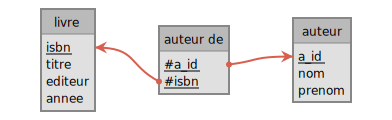
\includegraphics{https://raw.githubusercontent.com/padilla-nsi/tnsi/main/cours/donnees/2-basesDeDonneesRelationnelles/img3relations.png}
\caption{Schéma des 3 relations}
\end{figure}

    Le schéma de la relation \texttt{auteur\_de} est :

\[auteur\_de \qquad (\underline{a\_id}: Int , \underline{isbn}: String)\]

Comme on peut le voir ici, il faut mettre en place :

\begin{itemize}
\tightlist
\item
  une \textbf{clé primaire sur le couple (\texttt{a\_id},
  \texttt{isnb})} (car l'\texttt{isbn} tout seul ou l'\texttt{a\_id}
  tout seul ne rendent pas une entité de cette relation unique : un même
  isbn peut être associé à deux auteurs différents (et donc apparaître
  dans deux entités différentes) et un auteur peut écrire plusieurs
  livres (et donc peut apparaître dans de multiples entités). Ce qui est
  unique, c'est le couple (\texttt{a\_id}, `isbn).
\item
  deux \textbf{contrainte de référence}.
\end{itemize}

    Pour créer cette relation, on procède comme d'habitude mais après la
définitions des attributs, on va ajouter trois lignes :

\begin{itemize}
\tightlist
\item
  \texttt{PRIMARY\ KEY} pour indiquer la clé primaire suivie du couple
  \texttt{(a\_id,\ isbn)}
\item
  \texttt{FOREIGN\ KEY(a\_id)} pour indiquer que l'attribut
  \texttt{a\_id} possède une contrainte de référence, suivi du mot-clé
  \texttt{REFERENCE\ auteur(a\_id)} qui pointe vers l'attribut
  \texttt{a\_id} de la relation \texttt{auteur}.
\item
  \texttt{FOREIGN\ KEY(isbn)\ REFERENCE\ livre(isbn)} pour indiquer que
  l'attribut \texttt{isbn} possède une contrainte de référence en lien
  avec l'attribut \texttt{isbn} de la relation \texttt{livre}.
\end{itemize}

        {\scriptsize
    \begin{tcolorbox}[breakable, size=fbox, boxrule=1pt, pad at break*=1mm,colback=cellbackground, colframe=cellborder]
\prompt{In}{incolor}{ }{\boxspacing}
\begin{Verbatim}[commandchars=\\\{\}]
\PY{o}{\PYZhy{}}\PY{o}{\PYZhy{}} \PY{n}{en} \PY{n}{cas} \PY{n}{d}\PY{l+s+s1}{\PYZsq{}}\PY{l+s+s1}{erreur, décommenter...}
\PY{o}{\PYZhy{}}\PY{o}{\PYZhy{}}
\PY{o}{\PYZhy{}}\PY{o}{\PYZhy{}} \PY{n}{DROP} \PY{n}{TABLE} \PY{n}{IF} \PY{n}{EXISTS} \PY{n}{auteur\PYZus{}de}\PY{p}{;}
\end{Verbatim}
\end{tcolorbox}
    }

        {\scriptsize
    \begin{tcolorbox}[breakable, size=fbox, boxrule=1pt, pad at break*=1mm,colback=cellbackground, colframe=cellborder]
\prompt{In}{incolor}{ }{\boxspacing}
\begin{Verbatim}[commandchars=\\\{\}]
\PY{n}{CREATE} \PY{n}{TABLE} \PY{n}{auteur\PYZus{}de} \PY{p}{(}
    \PY{n}{a\PYZus{}id}    \PY{n}{INTEGER}\PY{p}{,}
    \PY{n}{isbn}    \PY{n}{TEXT}\PY{p}{,}
    \PY{n}{PRIMARY} \PY{n}{KEY} \PY{p}{(}\PY{n}{a\PYZus{}id}\PY{p}{,} \PY{n}{isbn}\PY{p}{)}\PY{p}{,}                    \PY{o}{\PYZhy{}}\PY{o}{\PYZhy{}} \PY{n}{clé} \PY{n}{primaire} \PY{n}{pour} \PY{n}{le} \PY{n}{couple}
    \PY{n}{FOREIGN} \PY{n}{KEY}\PY{p}{(}\PY{n}{a\PYZus{}id}\PY{p}{)} \PY{n}{REFERENCES} \PY{n}{auteur}\PY{p}{(}\PY{n}{a\PYZus{}id}\PY{p}{)}\PY{p}{,}   \PY{o}{\PYZhy{}}\PY{o}{\PYZhy{}} \PY{n}{clés} \PY{n}{étrangères} \PY{n}{et} \PY{n}{contraintes} \PY{n}{de} \PY{n}{référence}
    \PY{n}{FOREIGN} \PY{n}{KEY}\PY{p}{(}\PY{n}{isbn}\PY{p}{)} \PY{n}{REFERENCES} \PY{n}{livre}\PY{p}{(}\PY{n}{isbn}\PY{p}{)}     \PY{o}{\PYZhy{}}\PY{o}{\PYZhy{}}      \PY{n}{vers} \PY{n}{les} \PY{n}{relations} \PY{l+s+s1}{\PYZsq{}}\PY{l+s+s1}{auteur}\PY{l+s+s1}{\PYZsq{}} \PY{n}{et} \PY{l+s+s1}{\PYZsq{}}\PY{l+s+s1}{livre}\PY{l+s+s1}{\PYZsq{}}
\PY{p}{)}\PY{p}{;}
\end{Verbatim}
\end{tcolorbox}
    }

    Maintenant que la relation et ses contraintes sont définies, on peut
insérer des données.

Par exemple \texttt{Twain\ Mark} (a\_id: 0) est l'auteur de
\texttt{Les\ Aventures\ de\ Huckleberry\ Finn} (\texttt{isbn}:
978-2081509511)

        {\scriptsize
    \begin{tcolorbox}[breakable, size=fbox, boxrule=1pt, pad at break*=1mm,colback=cellbackground, colframe=cellborder]
\prompt{In}{incolor}{ }{\boxspacing}
\begin{Verbatim}[commandchars=\\\{\}]
\PY{n}{INSERT} \PY{n}{INTO} \PY{n}{auteur\PYZus{}de} \PY{n}{VALUES} \PY{p}{(}\PY{l+m+mi}{0}\PY{p}{,} \PY{l+s+s1}{\PYZsq{}}\PY{l+s+s1}{978\PYZhy{}2081509511}\PY{l+s+s1}{\PYZsq{}}\PY{p}{)}\PY{p}{;}
\end{Verbatim}
\end{tcolorbox}
    }

    \textbf{Pas de doublons} En revanche, impossible de saisir la meme fiche
en double :

        {\scriptsize
    \begin{tcolorbox}[breakable, size=fbox, boxrule=1pt, pad at break*=1mm,colback=cellbackground, colframe=cellborder]
\prompt{In}{incolor}{ }{\boxspacing}
\begin{Verbatim}[commandchars=\\\{\}]
\PY{n}{INSERT} \PY{n}{INTO} \PY{n}{auteur\PYZus{}de} \PY{n}{VALUES}\PY{p}{(}\PY{l+m+mi}{0}\PY{p}{,} \PY{l+s+s1}{\PYZsq{}}\PY{l+s+s1}{978\PYZhy{}2081509511}\PY{l+s+s1}{\PYZsq{}}\PY{p}{)}\PY{p}{;}    \PY{o}{\PYZhy{}}\PY{o}{\PYZhy{}} \PY{n}{erreur} \PY{n}{d}\PY{l+s+s1}{\PYZsq{}}\PY{l+s+s1}{unicitié de la clé primaire}
\end{Verbatim}
\end{tcolorbox}
    }

    \textbf{Plusieurs auteurs} Mais un livre peut avoir plusieurs auteurs
(car la clé primaire est le couple ! et non pas l'isbn tout seul).

Ici, c'est le livre \texttt{Astérix\ chez\ les\ Pictes} qui possède 4
auteurs différents :

        {\scriptsize
    \begin{tcolorbox}[breakable, size=fbox, boxrule=1pt, pad at break*=1mm,colback=cellbackground, colframe=cellborder]
\prompt{In}{incolor}{ }{\boxspacing}
\begin{Verbatim}[commandchars=\\\{\}]
\PY{n}{INSERT} \PY{n}{INTO} \PY{n}{auteur\PYZus{}de} \PY{n}{VALUES} 
    \PY{p}{(}\PY{l+m+mi}{5}\PY{p}{,} \PY{l+s+s1}{\PYZsq{}}\PY{l+s+s1}{978\PYZhy{}2864972662}\PY{l+s+s1}{\PYZsq{}}\PY{p}{)}\PY{p}{,}
    \PY{p}{(}\PY{l+m+mi}{6}\PY{p}{,} \PY{l+s+s1}{\PYZsq{}}\PY{l+s+s1}{978\PYZhy{}2864972662}\PY{l+s+s1}{\PYZsq{}}\PY{p}{)}\PY{p}{,}
    \PY{p}{(}\PY{l+m+mi}{7}\PY{p}{,} \PY{l+s+s1}{\PYZsq{}}\PY{l+s+s1}{978\PYZhy{}2864972662}\PY{l+s+s1}{\PYZsq{}}\PY{p}{)}\PY{p}{,}
    \PY{p}{(}\PY{l+m+mi}{8}\PY{p}{,} \PY{l+s+s1}{\PYZsq{}}\PY{l+s+s1}{978\PYZhy{}2864972662}\PY{l+s+s1}{\PYZsq{}}\PY{p}{)}\PY{p}{;}
\end{Verbatim}
\end{tcolorbox}
    }

    \textbf{Contrainte de référence} Et impossible de créer une fiche si la
référence n'existe pas.

Par exemple :

\begin{itemize}
\tightlist
\item
  Comme il n'y a pas d'auteur ayant pour \texttt{a\_id} la valeur
  \texttt{1000}, cette insertion est impossible.
\end{itemize}

        {\scriptsize
    \begin{tcolorbox}[breakable, size=fbox, boxrule=1pt, pad at break*=1mm,colback=cellbackground, colframe=cellborder]
\prompt{In}{incolor}{ }{\boxspacing}
\begin{Verbatim}[commandchars=\\\{\}]
\PY{n}{INSERT} \PY{n}{INTO} \PY{n}{auteur\PYZus{}de} \PY{n}{VALUES} \PY{p}{(}\PY{l+m+mi}{1000}\PY{p}{,} \PY{l+s+s1}{\PYZsq{}}\PY{l+s+s1}{978\PYZhy{}2864972662}\PY{l+s+s1}{\PYZsq{}}\PY{p}{)}    \PY{o}{\PYZhy{}}\PY{o}{\PYZhy{}} \PY{n}{erreur} \PY{p}{:} \PY{n}{contrainte} \PY{n}{de} \PY{n}{référence}
\end{Verbatim}
\end{tcolorbox}
    }

    Par exemple :

\begin{itemize}
\tightlist
\item
  Comme le livre d'isbn \texttt{123-1234567890} n'existe pas,
  l'insertion lève une erreur
\end{itemize}

        {\scriptsize
    \begin{tcolorbox}[breakable, size=fbox, boxrule=1pt, pad at break*=1mm,colback=cellbackground, colframe=cellborder]
\prompt{In}{incolor}{ }{\boxspacing}
\begin{Verbatim}[commandchars=\\\{\}]
\PY{n}{INSERT} \PY{n}{INTO} \PY{n}{auteur\PYZus{}de} \PY{n}{VALUES} \PY{p}{(}\PY{l+m+mi}{0}\PY{p}{,} \PY{l+s+s1}{\PYZsq{}}\PY{l+s+s1}{123\PYZhy{}1234567890}\PY{l+s+s1}{\PYZsq{}}\PY{p}{)}    \PY{o}{\PYZhy{}}\PY{o}{\PYZhy{}} \PY{n}{erreur} \PY{p}{:} \PY{n}{contrainte} \PY{n}{de} \PY{n}{référence}
\end{Verbatim}
\end{tcolorbox}
    }

    On peut maintenant insérer plus d'entités dans la relation :

        {\scriptsize
    \begin{tcolorbox}[breakable, size=fbox, boxrule=1pt, pad at break*=1mm,colback=cellbackground, colframe=cellborder]
\prompt{In}{incolor}{ }{\boxspacing}
\begin{Verbatim}[commandchars=\\\{\}]
\PY{n}{INSERT} \PY{n}{INTO} \PY{n}{auteur\PYZus{}de} \PY{n}{VALUES} 
    \PY{p}{(}\PY{l+m+mi}{1}\PY{p}{,} \PY{l+s+s1}{\PYZsq{}}\PY{l+s+s1}{978\PYZhy{}2207249123}\PY{l+s+s1}{\PYZsq{}}\PY{p}{)}\PY{p}{,}
    \PY{p}{(}\PY{l+m+mi}{2}\PY{p}{,} \PY{l+s+s1}{\PYZsq{}}\PY{l+s+s1}{978\PYZhy{}2723428262}\PY{l+s+s1}{\PYZsq{}}\PY{p}{)}\PY{p}{,}
    \PY{p}{(}\PY{l+m+mi}{3}\PY{p}{,} \PY{l+s+s1}{\PYZsq{}}\PY{l+s+s1}{978\PYZhy{}2745989857}\PY{l+s+s1}{\PYZsq{}}\PY{p}{)}\PY{p}{,}
    \PY{p}{(}\PY{l+m+mi}{4}\PY{p}{,} \PY{l+s+s1}{\PYZsq{}}\PY{l+s+s1}{978\PYZhy{}2745989857}\PY{l+s+s1}{\PYZsq{}}\PY{p}{)}\PY{p}{,}
    \PY{p}{(}\PY{l+m+mi}{9}\PY{p}{,} \PY{l+s+s1}{\PYZsq{}}\PY{l+s+s1}{978\PYZhy{}2221197691}\PY{l+s+s1}{\PYZsq{}}\PY{p}{)}\PY{p}{,}
    \PY{p}{(}\PY{l+m+mi}{10}\PY{p}{,} \PY{l+s+s1}{\PYZsq{}}\PY{l+s+s1}{978\PYZhy{}2335008586}\PY{l+s+s1}{\PYZsq{}}\PY{p}{)}\PY{p}{,}
    \PY{p}{(}\PY{l+m+mi}{11}\PY{p}{,} \PY{l+s+s1}{\PYZsq{}}\PY{l+s+s1}{978\PYZhy{}2335008586}\PY{l+s+s1}{\PYZsq{}}\PY{p}{)}\PY{p}{,}
    \PY{p}{(}\PY{l+m+mi}{12}\PY{p}{,} \PY{l+s+s1}{\PYZsq{}}\PY{l+s+s1}{978\PYZhy{}0141391601}\PY{l+s+s1}{\PYZsq{}}\PY{p}{)}\PY{p}{,}
    \PY{p}{(}\PY{l+m+mi}{13}\PY{p}{,} \PY{l+s+s1}{\PYZsq{}}\PY{l+s+s1}{978\PYZhy{}2258116429}\PY{l+s+s1}{\PYZsq{}}\PY{p}{)}\PY{p}{;}
\end{Verbatim}
\end{tcolorbox}
    }

        {\scriptsize
    \begin{tcolorbox}[breakable, size=fbox, boxrule=1pt, pad at break*=1mm,colback=cellbackground, colframe=cellborder]
\prompt{In}{incolor}{ }{\boxspacing}
\begin{Verbatim}[commandchars=\\\{\}]
\PY{n}{SELECT} \PY{o}{*} \PY{n}{FROM} \PY{n}{auteur\PYZus{}de}\PY{p}{;}
\end{Verbatim}
\end{tcolorbox}
    }

    \hypertarget{muxe9diathuxe8que-relations-usager-et-emrunt}{%
\subsection{\texorpdfstring{Médiathèque : relations \texttt{usager} et
\texttt{emrunt}}{Médiathèque : relations usager et emrunt}}\label{muxe9diathuxe8que-relations-usager-et-emrunt}}

    À toi de finir en ajoutant maintenant les relations \texttt{usager} puis
\texttt{emprunt} en suivant le schéma suivant :

(tous les attributs à ajouter sont des String)

    \begin{figure}
\centering
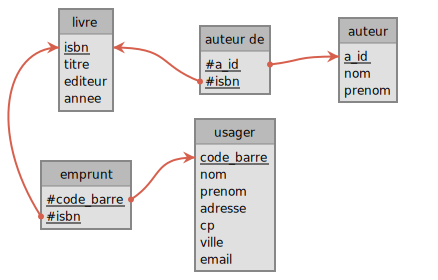
\includegraphics{https://raw.githubusercontent.com/padilla-nsi/tnsi/main/cours/donnees/2-basesDeDonneesRelationnelles/img5relations.png}
\caption{Schéma des 5 relations}
\end{figure}

        {\scriptsize
    \begin{tcolorbox}[breakable, size=fbox, boxrule=1pt, pad at break*=1mm,colback=cellbackground, colframe=cellborder]
\prompt{In}{incolor}{ }{\boxspacing}
\begin{Verbatim}[commandchars=\\\{\}]

\end{Verbatim}
\end{tcolorbox}
    }


    % Add a bibliography block to the postdoc
    
    
    
\end{document}
